\documentclass[a4paper,12pt]{article}
\usepackage{graphicx}
\usepackage{amsmath}
\usepackage{geometry}
\usepackage{float}
\usepackage{tikz}

\providecommand{\brak}[1]{\ensuremath{\left(#1\right)}}
\geometry{margin=1in}

\title{Clock}
\author{EE24BTECH11005: Credits EE24BTECH11001, EE24BTECH11002}
\date{\today}

\begin{document}

\maketitle

\section*{Introduction}
This project showcases an innovative clock design implemented on the AtMega328p microcontroller using the avr-gcc framework. The primary focus was on achieving maximum time accuracy. To optimize performance, time incrementation was implemented using Karnaugh maps (K-maps) instead of conventional increment commands. The entire codebase was meticulously crafted in AVR Assembly language, allowing precise control over instruction execution times and enabling fine-tuned timing adjustments.

\section*{Overview}
\subsection*{Features}
The main features of the calculator are,
\begin{itemize}
    \item The entire code was written in AVR Assembly so it is very $bare-bones$ so more focus was placed on making the clock accurate than adding more and more functionality.
    \item Instead of using $\mathbf{inc}$ command, k-maps were used. 
    \item The use of one decoder for each 7-segment display was avoided (only one decoder was used).

\end{itemize}
\subsection*{Hardware Overview}


The hardware consists of:
\begin{table}[H]
\centering
\begin{tabular}{|c|l|}
\hline
\textbf{Quantity} & \textbf{Component} \\
\hline
6 & 7 Segment Display \\
\hline
1 & Arduino Uno\\
\hline
- & Wires \\
\hline
1 & Decoder (7447) \\
\hline
\end{tabular}
\caption{Materials Required}
\label{tab:materials}
\end{table}

\begin{itemize}
    \item Decrease requirement of multiple decoders, by intelligentally connecting the circuit as shown in the schematic
    Figure~\ref{fig:circuit_schematic}.
\end{itemize}
The schematic for connections is as shown below,
\begin{figure}[H]
    \centering
    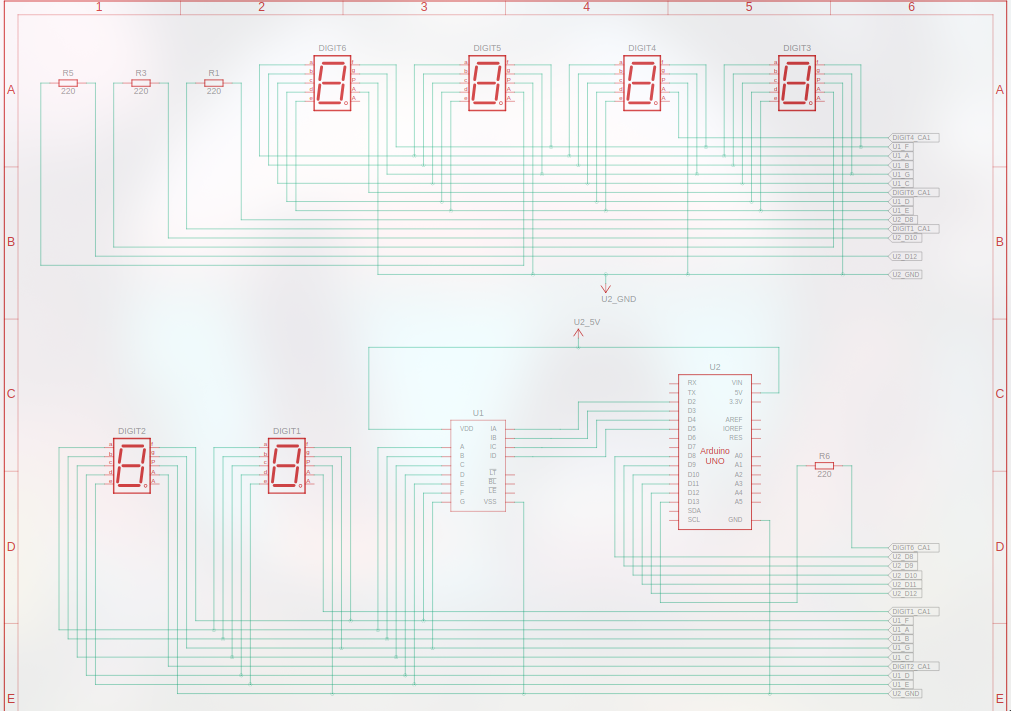
\includegraphics[width=\textwidth]{figs/circuit_schematic.png}
    \caption{Schematic of Circuit.}
    \label{fig:circuit_schematic}
\end{figure}
\subsection*{Software Overview}
The software is implemented using AVR Assembly. It includes:
\begin{itemize}
    \item Using k-maps for implementing
    \item Timer was implemented through repeated looping
    \item Registers were intelligently used so that code was implemented using only the $16$ provided registers (r15, r30)
\end{itemize}
Now let us explore some of the features mentioned above in greater depth.
\section*{In Depth}
\subsection*{Karnaugh Maps}

\subsubsection*{K-map 1}
This is for one's digit of seconds, minutes, \newline \newline
\begin{tabular}{|c|c|}
\hline
WXYZ & ABCD \\
\hline
0000 & 0001 \\
0001 & 0010 \\
0010 & 0011 \\
0011 & 0100 \\
0100 & 0101 \\
0101 & 0110 \\
0110 & 0111 \\
0111 & 1000 \\
1000 & 1001 \\
1001 & 1010 \\
\hline
\end{tabular}
\newline
\newline These are the K-maps for $A, B, C, D$
\begin{align*}
A &= \overline{W} \\
B &= (\overline{W} \& X \& \overline{Z})  ||  (W \& \overline{X} \& \overline{Z}) \\
C &= (\overline{W} \& Y \& \overline{Z})  ||  (\overline{X} \& Y \& \overline{Z}) || (W \& X \& \overline{Y} \& \overline{Z}) \\
D &= (W \& X \& Y \& \overline{Z})  ||  (\overline{W} \& \overline{X} \& \overline{Y} \& Z)
\end{align*}
\subsubsection*{K-map 2}
This is for ten's digit of minutes, seconds, \newline \newline
\begin{tabular}{|c|c|}
\hline
WXYZ & ABCD \\
\hline
0000 & 0001 \\
0001 & 0010 \\
0010 & 0011 \\
0011 & 0100 \\
0100 & 0101 \\
0101 & 0000 \\0011 & 0100 \\
0100 & 0101 \\
0101 & 0000 \\
\hline
\end{tabular}
\newline
\newline These are the K-maps for $A, B, C, D$
\begin{align*}
A &= 0 \\
B &= (\overline{X} \& Y \& Z) || (X \& \overline{Y} \& \overline{Z}) \\
C &= (\overline{X} \& \overline{Y} \& Z) || (\overline{X} \& Y \& \overline{Z}) \\
D &= (\overline{X} \& Y \& \overline{Z}) || (\overline{X}\& \overline{Y} \& \overline{Z})
\end{align*}
\subsubsection*{K-map 3}
This is for one's digits of hours, \newline \newline
\begin{tabular}{|c|c|}
\hline
WXYZ & ABCD \\
\hline
0000 & 0001 \\
0001 & 0010 \\
0010 & 0000 \\
\hline
\end{tabular}
\newline
\newline These are the K-maps for $A, B, C, D$
\begin{align*}
A &= 0 \\
B &= 0 \\
C &= (\overline{Y} \& Z) \\
D &= (\overline{Y} \& \overline{Z})
\end{align*}
\subsubsection*{K-map 4}
This is for ten's digits of hours, \newline \newline
\begin{tabular}{|c|c|}
\hline
WXYZ & ABCD \\
\hline
0000 & 0001 \\
0001 & 0000 \\
\hline
\end{tabular}
\newline
\newline These are the K-maps for $A, B, C, D$
\begin{align*}
A &= 0 \\
B &= 0 \\
C &= 0 \\
D &= \overline{Z}
\end{align*}
\subsection*{Timer}
Using multiple loops, a timer of one second was created. Within that one second, time is displayed (using the logic mentioned above), and at the end of one second, one's digit is incremented. The sub routine that does this has a piece of code at the end to increment ten's digit of seconds if incremented value of one's digit is 0. Similar the function to increment ten's digit has a line of code to increment one's digit of minutes if value after incrementing is 0. This is how time is incremented

\section*{Conclusion}
This project has demonstrated my attempt to implement a fully functional timer using 7 segment displays, a decoder, and an AtMega328p microcontroller (arduino uno) implemented using AVR Assembly and Karnaugh Maps. 

\end{document}
